%
\documentclass[12pt]{ociamthesis}
\usepackage{tikz}
\newcommand{\id}{\mathrm{id}}
\begin{document}

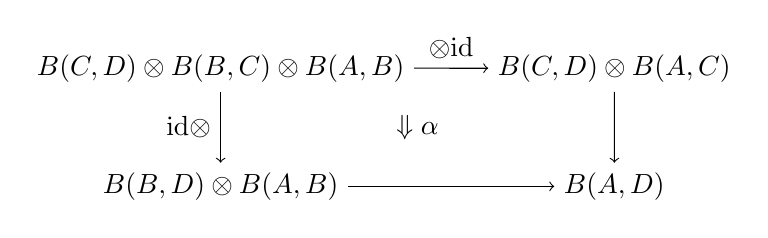
\begin{tikzpicture}[yscale=1.5, xscale=2.5]
\node (A) at (0,1){${\cat B}(C,D) \otimes {\cat B}(B, C) \otimes {\cat B}(A,B)$};
\node (C) at (2,1){${\cat B}(C,D) \otimes {\cat B}(A,C)$};
\node (D) at (0,0) {${\cat B}(B,D)  \otimes {\cat B}(A,B)$};
\node (E) at (2,0) {${\cat B}(A, D) $};
\node (B) at (1,.5) {$\Downarrow \alpha$};
\draw[->] (A) to node[above]{$\comp \otimes \id$} (C);
\draw[->] (A) to node[left]{$\id \otimes \comp$} (D);
\draw[->] (C) to node[right]{$\comp$} (E);
\draw[->] (D) to node[above]{$\comp$} (E);
\end{tikzpicture}
\end{document} 
